\documentclass[conference,9pt,final]{./../Templates/IEEEtran5/IEEEtran}


%\usepackage[margin=2cm]{geometry}
\usepackage[ruled,vlined]{algorithm2e}

\usepackage{dsfont}
\usepackage[cmex10]{mathtools}
\usepackage[dvips]{graphicx}

\usepackage{setspace}
\usepackage[cmex10]{amsmath}
\usepackage{mdwmath}
\usepackage{mdwtab}
\usepackage{acronym}
\usepackage{xfrac}
\usepackage{amsfonts}


\acrodef{MU-MIMO}{\ac{MU} \ac{MIMO}}
\acrodef{SU-MIMO}{\ac{SU} \ac{MIMO}}
\acrodef{SU}{single-user}
\acrodef{MU}{multi-user}
\acrodef{MIMO}{multiple-input multiple-output}
\acrodef{SP}{successive projections}
\acrodef{AHP}{analytic hierarchy process}
\acrodef{M-AHP}{modified analytic hierarchy process}
\acrodef{MMSE}{minimum mean squared error}
\acrodef{EVD}{eigen-value decomposition}
\acrodef{SVD}{singular value decomposition}
\acrodef{GS}{Gram-Schmidt}
\acrodef{RNS}{reduced null space}
\acrodef{ZF}{zero-forcing}
\acrodef{SUS}{semi-orthogonal user selection}
\acrodef{BD}{block diagonalization}
\acrodef{RR}{round-robin}
\acrodef{RAT}{radio access technologies}
\acrodef{W-MMSE}{weighted minimum mean squared error}
\acrodef{S-US}{static user selection}
\acrodef{C-US}{coordinated user selection}
\acrodef{DoF}{degrees of freedom}
\acrodef{BF}{beamforming}
\acrodef{BS}{base station}
\acrodef{WF}{water-filing}
\acrodef{SINR}{signal to interference and noise ratio}
\acrodef{SNR}{signal to noise ratio}
\acrodef{PHY}{physical}
\acrodef{MAC}{medium access control}
\acrodef{PF}{proportional fair}
\acrodef{QoS}{quality of service}
\acrodef{SLNR}{signal to leakage noise ratio}
\acrodef{WSRM}{weighted sum rate maximization}
\acrodef{QRD}{QR decomposition}
\graphicspath{{./../Figures/}}
\DeclareGraphicsExtensions{.eps}

%\doublespacing

\title{Iterative Scheduling for Cell-Edge in Multi-Cell MU-MIMO}
\author{\IEEEauthorblockN{Ganesh Venkatraman, Antti T\"{o}lli, Janne Janhunen and Markku Juntti}
\IEEEauthorblockA{Center for Wireless Communications (CWC), University of Oulu, Oulu, FI-90014\\
Email: \{gvenkatr, antti.tolli, janne.janhunen, markku.juntti\}@ee.oulu.fi}
}


\begin{document}

\maketitle

% Text related command shortcuts

\newcommand{\bi}[1]{\textbf{\textit{#1}}}

% Math related command shortcuts

\newcommand{\mbi}[1]{\mathbf{\mathit{#1}}}
\newcommand{\mbf}[1]{\mathbf{#1}}

\newcommand{\mscrmxy}[2]{{#1}_{\mathrm{#2}}}
\newcommand{\msclxy}[2]{{#1}_{\mathit{#2}}}
\newcommand{\msclxyz}[3]{{#1}_{\mathit{#2},\mathit{#3}}}

\newcommand{\mvecnxy}[2]{\mathbf{#1}_{#2}}
\newcommand{\mvecnxyz}[3]{\mathbf{#1}_{#2,#3}}
\newcommand{\mvecxy}[2]{\mathbf{#1}_{\mathit{#2}}}
\newcommand{\mvecxyz}[3]{\mathbf{#1}_{\mathit{#2},\mathit{#3}}}

\newcommand{\me}[1]{\(#1\)}
\newcommand{\mrm}[1]{\mathrm{#1}}
\newcommand{\mc}[1]{\mathcal{#1}}
\newcommand{\mtext}[1]{\mathit{#1}}

\newcommand{\mxu}[2]{\mathbf{#1}^{\mathit{#2}}}
\newcommand{\mxl}[2]{\mathbf{#1}_{\mathit{#2}}}
\newcommand{\mxul}[3]{\mathbf{#1}^{\mathit{#2}}_{\mathit{#3}}}

\newcommand{\inm}{\, \in \,}
\newcommand{\fall}{\, \forall \,}
\newcommand{\bs}{\: \backslash \:}
\newcommand{\card}[1]{| \, #1 \, |}
\newcommand{\norm}[2]{\|\, #1 \,\|_{#2}}
\newcommand{\gnorm}[1]{\|\, #1 \,\|}
\newcommand{\sset}{\, \subset \,}

\newcommand{\inmt}[1]{\( \mathit{#1} \)}
\newcommand{\mcxy}[2]{\mathcal{#1}_{\mathit{#2}}}

\newcommand{\matbcont}[1]{\left ( \, #1 \, \right )}
\newcommand{\matscont}[1]{\left [ \, #1 \, \right ]}
\newcommand{\setcont}[1]{\lbrace \, #1 \, \rbrace}

\newcommand{\argmax}{\operatorname*{\arg\,max}}

% Math environment command shortcuts

\newenvironment{ceq}{\begin{center}\begin{equation}}{\end{equation}\end{center}}
\newenvironment{cneq}{\begin{center}\begin{equation*}}{\end{equation*}\end{center}}

\newenvironment{ceqn}{\begin{center}\begin{eqnarray}}{\end{eqnarray}\end{center}}
\newenvironment{cneqn}{\begin{center}\begin{eqnarray*}}{\end{eqnarray*}\end{center}}


\begin{abstract}
The paper addresses the iterative joint scheduling algorithms for the cooperative multi-cell \ac{MU} \ac{MIMO} scheme with the sum rate maximization objective for the cell-edge users. The \ac{QRD} scheduling, which provides near-optimal scheduling for the single-cell users, suffers significantly when performed over the cell-edge users in the multi-cell scenario. In order to improve the cell-edge user selection, we propose an iterative \ac{S-US} scheduling scheme which selects the users jointly by minimizing the interference to the neighboring \ac{BS} users. The proposed scheme provides better performance over the \ac{QRD} scheme by sharing the available \ac{DoF} with the coordinating \ac{BS}s. The extension to the \ac{S-US} scheme, namely \ac{C-US} scheme, which selects the user and the associated \ac{BS} jointly from the common user pool is discussed in the context of coordinated multi-point transmission. The simulation figures are provided in comparison with the existing scheduling schemes for the sum rate maximization objective.

\end{abstract}

\acresetall

\section{Introduction}


The scheduling of the users for \ac{MU} \ac{MIMO} transmission requires the knowledge of the channel conditions of each user in order to achieve considerable gain over \ac{SU} \ac{MIMO}. The \ac{MU}-\ac{MIMO} transmission requires user channel vectors to be linearly independent to provide interference-free transmission for the multiplexed users with the help of precoders.

There are numerous papers discussing the scheduling of users for \ac{MU}-\ac{MIMO} transmission with the \ac{ZF} \ac{BF} design. The precoder design based on \ac{ZF}-\ac{BF} provides efficient de-coupling of the transmitted streams at the receiver by zeroing the interference caused by other streams over the desired channel \cite{spencer2004zero,wiesel2008zero}. The precoders are designed for the set of users whose data streams are to be multiplexed at the given scheduling instant. The \ac{MU}-\ac{MIMO} user set is identified from the available pool of users based on \ac{QoS} constraints and the linear independency of the channel vectors.
The selection of users based on linearly independent channel vectors were well studied in the literature. The selection based on the \ac{GS} algorithm as \ac{SUS} algorithm was discussed in \cite{sus2006zfbf} and the extension with the multi-antenna receivers as considered in \cite{antti_user_selection}.  Algorithms using \ac{BD} of the stacked channel vectors by successively projecting onto the null space as discussed in \cite{shen2006low} and \cite{youtuan2007improved}. Selection of users based on stochastic algorithms were considered in \cite{genetic_search} using \ac{PF} or sum rate maximization objectives. The user selection using the channel volume enclosure were considered in the scheduling for \ac{MU-MIMO} in \cite{ko2012determinant} and \cite{jin2010novel}. The selection based on volume enclosure provides similar selection based on \ac{SUS} algorithm.

The joint precoder design and scheduling were carried out for \ac{MU}-\ac{MIMO} transmission using the interference leakage formulation \cite{sadek} and \cite{leakage}. The selection was carried out in a greedy manner using the \ac{SLNR} metric and the precoders were designed based on the maximum eigen-vector of the matrices involved \ac{SLNR} calculation. The iterative precoder design considered in \cite{traniterative} was based on the \ac{BD} of the channel vectors of stacked user channels and the precoders were designed after each selection. The precoder design using \ac{W-MMSE} equivalent for \ac{WSRM} was considered using the alternating optimization method for obtaining the precoder in an iterative manner. The overloaded design in which the number of users are greater than the available spatial \ac{DoF}, the \ac{W-MMSE} scheme performs joint scheduling and the precoder design by providing zero powered precoders for nonscheduled users \cite{wmmse_shi}.

This paper discusses the joint scheduling of cell-edge users across multi-cell scenario in an iterative manner to provide interference-free transmission. Since the users are at the cell-edge are interference limited, the available spatial \ac{DoF} are shared across the transmission user sets of all \ac{BS}s. The proposed joint scheduling schemes are compared with other joint scheduling and precoder design schemes in the literature. The proposed schemes provides a way to use the simple \ac{ZF}-\ac{BF} based precoders to achieve similar performance as of \ac{W-MMSE} scheme.


\section{System Model}

We consider the downlink transmission with a \me{N_\mrm{B}} \ac{BS}, having \me{N_\mrm{T}} transmit antennas and \me{K} users each with a single receive antenna. Let \me{\mc{B}} represent the set of \ac{BS} indices and the user indices associated with the \ac{BS} \me{b} is denoted as \me{\mc{U}_b \fall b \inm \mc{B}}. The received signal \me{\msclxyz{y}{b}{k}} of user \me{k} associated to \ac{BS} \me{b} is given by
%\begin{eqnarray}
%\msclxyz{y}{b}{k} =& \overbrace{\mvecxyz{h}{b}{k} \mvecxyz{x}{b}{k}}^{\mathclap{\text{desired term}}} \quad + \quad \overbrace{ \mvecxyz{h}{b}{k} \sum_{\mathclap{\mtext{i} \inm \mc{S}_b \bs \mtext{k}}} \mvecxyz{x}{b}{i}}^{\mathclap{\text{intra-cell interference terms}}} \nonumber \\
% & + \quad \underbrace{ \sum_{\mathclap{\mtext{s} \inm \mc{B} \bs b}} \mvecxyz{h}{s}{k} \sum_{\mathclap{\mtext{j} \inm \mc{S}_s}} \mvecxyz{x}{s}{j}}_{\mathclap{\text{inter-cell interference terms}}} \quad + \quad \msclxyz{n}{b}{k}
%\label{sm-e1}
%\end{eqnarray}
\begin{eqnarray}
\msclxyz{y}{b}{k} = \underbrace{\mvecxyz{h}{b}{k} \mvecxyz{x}{b}{k}}_{\mathclap{\text{desired term}}} \quad + \quad \overbrace{\sum_{\mathclap{s \inm \mc{B}}} \mvecxyz{h}{s}{k} \quad \sum_{\mathclap{i \inm \mc{S}_s \bs k \inm b}} \mvecxyz{x}{s}{i}}^{\mathclap{\text{interfering terms}}} \quad + \quad \msclxyz{n}{b}{k},
\label{sm-e1}
\end{eqnarray}
where vector \me{\mvecxyz{x}{b}{k} \inm \mathds{C}^{\mscrmxy{N}{T}}} represents the transmitted symbol for user \me{k} from \ac{BS} \me{b}, noise \me{\msclxyz{n}{b}{k} \sim \mc{CN}(0,\mtext{N}_0)} is circularly symmetric and complex Gaussian, the channel \me{\mvecxyz{h}{b}{k} \inm \mathds{C}^{1 \times \mscrmxy{N}{T}}} between \ac{BS} \me{b} and the user \inmt{k} with each entries drawn from \me{\sim \mc{CN}(0,\mbf{I}_{N_\mrm{T}})}, and \me{\mvecxyz{h}{s}{k} \inm \mathds{C}^{1 \times \mscrmxy{N}{T}}} denotes the channel seen by the user \me{k \inm \mc{U}_b} and the neighboring \ac{BS} \me{s}. The set \me{\mc{S}_b \subset \mc{U}_b} represents the set of user indices grouped for the current transmission instant which is determined based on the scheduling scheme for the \ac{BS} \me{b}. The transmitted symbol \me{\mvecxyz{x}{b}{k}} for the user \inmt{k} from \ac{BS} \me{b} is given as \me{\mvecxyz{x}{b}{k} = \mvecxyz{m}{b}{k} \, \msclxyz{d}{b}{k}}, where \me{\mvecxyz{m}{b}{k}} is the precoder assigned to the user \inmt{k}, and \me{\msclxyz{d}{b}{k}} represents the data for the \inmt{k^{\mtext{th}}} user with \me{\mbf{E} [\, \card{d}^2 ] = 1}. The total transmit power
\begin{equation}
\sum_{k \inm \mc{S}_b} \mrm{Tr} \left ( \mvecxyz{m}{b}{k} \, \mvecxyz{m}{b}{k}^{\mrm{H}} \right ) \leq \mrm{P}_{t} \; \fall b \inm \mc{B}
\label{sm-e2}
\end{equation}
is limited by \me{\mrm{P}_{t}} for each \ac{BS} in the system.

The precoder \me{\mvecxyz{m}{b}{k}}, which decouples the transmitted data \me{\msclxyz{d}{b}{k}}, is given by the simple \ac{ZF}-\ac{BF} scheme \cite{spencer2004zero} or by designing with \ac{W-MMSE} as discussed in \cite{wmmse_shi}. The \ac{ZF}-\ac{BF} design provides interference free transmission by inverting the augmented channel matrix formed by stacking the channel vectors of users in the transmission set of all coordinating \ac{BS}s \me{\mc{S}_s \fall s \inm \mc{B}}. The stacked channel matrix of the \ac{BS} \me{b} is given by
\begin{eqnarray}
\mbf{H}_b = \matscont{\mvecnxyz{h}{b}{\mc{S}_{\mc{B}(1)}(1)}^\mrm{T} \quad \mvecnxyz{h}{b}{\mc{S}_{\mc{B}(1)}(2)}^\mrm{T} \, \dotsc \, \mvecnxyz{h}{b}{\mc{S}_{\mc{B}(N_\mrm{B})}(\card{\mc{S}_{\mc{B}(N_\mrm{B})}})}^\mrm{T} }, \label{sm-e3}
\end{eqnarray}
where \me{\mc{S}_{\mc{B}(i)}(j)} represent the \me{j^\mrm{th}} user in the transmission set of \me{i^\mrm{th}} \ac{BS} and the precoding vector \me{\mvecxyz{m}{b}{k}} is given by the corresponding column vector of the matrix \me{\mbf{M}} given by
\begin{equation}
\mbf{M} = \matscont{\dotsc \, \mvecnxyz{m}{b}{\mc{S}_b(1)} \, \dotsc \, \mvecnxyz{m}{b}{\mc{S}_b(k)} \, \dotsc \,} = (\mbf{H}^\mrm{H}_b \mbf{H}_b)^{-1}\mbf{H}^\mrm{H}_b.
\label{sm-e4}
\end{equation}

The power allocation is based on \ac{WF} principle which maximizes the sum rate by dividing power across the users
\begin{equation}
\msclxyz{p}{b}{k} = \matscont{\frac{1}{\lambda} - \gnorm{\mvecxyz{m}{b}{k}}^2 \; \mtext{N}_{0}}^+ \fall k \inm \mc{S}_b,
\label{sm-e5}
\end{equation}
where \me{\lbrace x \rbrace^+ \equiv \max(0,x)} and
\begin{equation}
\mvecxyz{m}{b}{k} = \msclxyz{p}{b}{k} \, \frac{\mvecxyz{m}{b}{k}}{\gnorm{\mvecxyz{m}{b}{k}}}
\label{sm-e6}
\end{equation}
represents the precoder for user \me{k \inm \mc{S}_b} with \me{\lambda \geq 0} is the dual variable for the sum power constraint \eqref{sm-e2}.


%\section{Single BS User Scheduling} \label{sbus}

%The scheduling schemes for single BS scenario are discussed briefly with a background note on the existing algorithms followed with the proposed algorithms.

%\subsection{Existing User Selection}

%
The user selection for MU-MIMO requires the channel vectors of the transmission set to be as orthogonal as possible in order to achieve the multiplexing gain. The selection of \me{\card{\mc{S}} \leq N_\mrm{T}} requires an exhaustive search of \me{\leq {^K C _{N_\mrm{T}}}} order complexity. Near-optimal schemes for determining the set \me{\mc{S}} were proposed in \cite{dimic2005downlink,shen2006low,antti_user_selection,sus2006zfbf,zhang2007user}. They are based on successive projection over the already chosen user set.

The selection process is initialized by picking the user with the maximum channel norm. The successive users are then identified at each iteration by selecting the user with the maximum projection onto the null space formed with the channel vectors of users in \me{\mc{S}}. At each iteration, \me{\card{S}} is updated with the user selected with the maximum norm and \eqref{sm-e3:1} is also updated accordingly to evaluate the null space \eqref{mca3-e1} for the next iteration. The procedure terminates when the condition \me{\card{\mc{S}} = N_\mrm{T}} is met. The condition corresponds to the limiting multiplexing gain available with \me{N_\mrm{T}} transmit antennas.

The null space of the channel vectors of user indices in the set \me{\mc{S}} is obtained by
\begin{eqnarray}
\mbf{N}(\mc{S}) &=& \mbf{I} - \mbf{H}^\mrm{H} ( \, \mbf{H} \mbf{H}^\mrm{H} \, )^{-1} \mbf{H}
\label{mca3-e1}
\end{eqnarray}
with \me{\mbf{H}} as given by \eqref{sm-e3:1}. At each iteration, the user \me{j} is selected based on the following objective
\begin{equation}
j = \arg \max_i \gnorm{\mvecxy{h}{i} \, \mbf{N}(\mc{S})} \, \fall i \inm \mc{U} \bs \mc{S}.
\label{mca3-e2}
\end{equation}

The selection scheme discussed in \cite{jin2010novel,ko2012determinant} provides an alternative interpretation of the successive projections discussed in \cite{dimic2005downlink,shen2006low,antti_user_selection,sus2006zfbf,zhang2007user}. Instead of maximizing the projection gain over the null space, the volume subtended by the channel vectors of users in \me{\mc{S}} and the channel vector of user \me{k \inm \mc{U} \bs \mc{S}} was evaluated. The channel vector of the user, which encloses the maximum volume with the vectors of users in \me{\mc{S}}, is chosen at the end of the current iteration. The above procedure is followed till the limiting size on \me{\mc{S}} was achieve as discussed earlier.

The complexity analysis of \ac{SP} scheme is discussed briefly. The number of complex multiplications involved in selecting the first user is \me{\varphi = K \, N_\mrm{T}}, which is attributed to the norm of the channel vectors. The remaining users are selected by projecting on to the null space of the users in \me{\mc{S}}. The null space of the chosen set of users has \me{N_\mrm{T} \times (q - 1)} dimensions and \me{q} represents the iteration index or \me{\card{\mc{S}}}. The complex multiplication involved in evaluating \eqref{mca3-e1} is given as \me{\xi(x) = x^2 \, N_\mrm{T} + O(x^3) + x \, N_\mrm{T} \, (N_\mrm{T} + x) } where \me{x} represents the number of channel vectors in \me{\mbf{H}} and \me{O(x^3)} represents the complexity involved with the inverse calculation for the matrix sized \me{x = q} at each iteration. The complexity involved is in the order of
\begin{eqnarray*}
\zeta_1 = O \left ( \varphi + \sum^{N_\mrm{T}}_{q = 2} \underbrace{N_\mrm{T}(1 + N_\mrm{T}) \, (K - q + 1)}_{\mathclap{\text{projection and norm for each user}}} + \xi(q - 1) \right )
\end{eqnarray*}


%\subsection{AHP based User Selection}

%
The \ac{SP} based user selection \cite{dimic2005downlink,shen2006low,antti_user_selection,sus2006zfbf,zhang2007user} provides efficient multiplexing by selecting a set of users with most linearly independent channel vectors. The selection procedure select the users in a greedy way at each instant. Let \me{i,j} be the indices of two users whose projection onto the null space \eqref{mca3-e1} yields the same metric value. It would be wiser to choose the user whose channel is well separated from the remaining user set \me{\mc{U} \bs \{ \mc{S} \cup k \}} with \me{k} being either \me{i} or \me{j} as discussed in \cite{wmmse_shi}. The \ac{AHP} scheme performs selection by considering the channel separation over the set \me{\mc{U} \bs \mc{S}} apart from considering \me{\mc{S}}.

The \ac{AHP} is a systematic procedure to select the best alternatives from the set of alternatives based on certain goals to be attained. The \ac{AHP} quantifies the alternatives with the priority metric which ranges between \me{[0,1]} with \me{1} representing the highest priority \cite{saaty2008decision}. The \ac{AHP} is used in the decision making process where the objective is to choose an alternative with the given constraints. The \ac{AHP} based procedure is utilized to select a user from the set \me{\mc{U}} with the objective of increasing the sum rate over the existing users in the set \me{\mc{S}}.

The \ac{AHP} procedure begins by formulating the pairwise symmetric matrix \me{\mbf{P}}, where each entry \me{\msclxyz{P}{i}{j}} should represent the pairwise relation between the users in \me{i^{\mrm{th}}} row and \me{j^{\mrm{th}}} column. Since the capacity is proportional to the volume enclosed between the channel vectors of user \me{i} and \me{j} \cite{ko2012determinant}, volume can be used as a metric to quantify the gain in multiplexing users \me{i} and \me{j}. The multiplexing gain between user \me{i} and \me{j} should include the vectors of users in \me{\mc{S}}, since they are already chosen in the previous iterations.

The selection procedure is initialized with the set \me{\mc{S} = \emptyset}, which is updated with the users at each iteration based on the selection criterion discussed below. The entry \me{\msclxyz{P}{i}{j}} denotes the volume of the user channel vectors \me{i^\mrm{th}} and \me{j^\mrm{th}} as given by \eqref{mca1-e1:1}
\begin{eqnarray}
\mbf{S} &=& \matscont{\mbf{H}^\mrm{T} \; \mvecxy{h}{i}^\mrm{T} \; \mvecxy{h}{j}^\mrm{T}} \\
\msclxyz{P}{i}{j} &=& \det{\left ( \, \mbf{S}^{\mrm{H}} \; \mbf{S} \, \right )} \label{mca1-e1:1}
\label{mca1-e1}
\end{eqnarray}
where \me{\mbf{H}^\mrm{T}} represents the stacked channel vectors of users in the set \me{\mc{S}} as given by \eqref{sm-e3:1}. The volume subtended by the column vectors of \me{\mbf{S}} is given by the determinant of the inner product \me{\mbf{S}^\mrm{H} \mbf{S}} which provides a measure of independency. The entry \me{\msclxyz{P}{i}{i}} corresponds to the diagonal entry of \me{\mbf{P}} represents the metric corresponds to the volume subtended between the channel vectors of users in \me{\mc{S}} and the \me{i^\mrm{th}} user as given by
\begin{eqnarray}
\mbf{S} &=& \matscont{\mbf{H}^\mrm{T} \; \mvecxy{h}{i}^\mrm{T}}
\label{mca1-e2}
\end{eqnarray}
where \me{\msclxyz{P}{i}{i}} is given by \eqref{mca1-e1:1} with \me{j = i}.

Matrix \me{\mbf{P}} of size \me{K \times K} represents the pairwise matrix with each entry updated with the volume formed between the already chosen set \me{\mc{S}} and the channel vector of users indexed by the row-column index. In order to find the candidate user for the set \me{\mc{S}} in the current iteration, the priorities for the users need to be evaluated based on capacity maximizing objective. The priorities among the users are given by the dominant eigen-vector of the matrix \me{\mbf{P} \succeq 0} \cite{saaty2008decision}. Let \me{\mbf{E} \mbf{\Lambda} \mbf{E}^\mrm{H}} be the eigen-value decomposition (EVD) of the matrix \me{\mbf{P}} and \me{\mvecxy{e}{\lambda_{\max}}} be the eigen-vector corresponding to the eigen-value \me{\lambda_{\max} \geq \lambda_i \fall \, \Lambda(i,i)} where \me{\mbf{\Lambda}} is the diagonal matrix with the eigen-values as the entries. The selection of user \me{i} is and the set update is given as
\begin{eqnarray}
i &=& \arg \max_{\mathrm{j}} |\;\msclxy{e}{\lambda_{\max}}(j)\;| \label{mca1-e3:1} \\
\mc{S} &=& \left \lbrace \, \mc{S} \, \cup \, i \, \right \rbrace.
\label{mca1-e3}
\end{eqnarray}

Selection is carried out in an iterative manner with the stopping criterion given by \me{\card{\mc{S}} = N_\mrm{T}} as detailed in Algorithm. \ref{mca1-a1}. Precoding is performed over the channels of the users in \me{\mc{S}} which forms the transmission set.
\begin{algorithm}
 \SetAlgoLined
 \DontPrintSemicolon
 \KwIn{\me{\mvecxy{h}{j} \fall j \inm \mc{U} }}
 \KwData{\me{\mc{S} = \emptyset, \, \mbf{P}, \, \mbf{H} = [\,]}}
 \While{\me{\card{S} \leq N_\mrm{T}}}{
 \ForEach{\me{ \msclxyz{P}{i}{j}, \, \mrm{where } \, i,j \inm \mc{U} \bs \mc{S}}}{
 formulate \me{\msclxyz{P}{i}{j}} using \eqref{mca1-e1:1} \;
 }
 perform EVD as \me{\mbf{M} = \mbf{E} \, \mbf{\Lambda} \, \mbf{E}^\mrm{H}} \;
 select user \me{i} using \eqref{mca1-e3:1} \;
 \me{\mc{S} = \{ \, \mc{S} \cup i \, \}}, \me{\mbf{H} = \matscont{\mbf{H}^\mrm{T} \; \mvecxy{h}{i}^\mrm{T}}^\mrm{T}} \;
 }
 \caption{AHP based User Selection}
 \label{mca1-a1}
\end{algorithm}

The diagonal entries of \me{\mbf{P}} requires \me{\varphi_1(x) = x^2 \, N_\mrm{T} + O(x^3)} and off-diagonal entries require \me{\varphi_2(x) = (x + 1)^2 N_\mrm{T} + O((x + 1)^3)} complex multiplications with \me{x} being the size of the square matrix \me{\mbf{P}} formed at each iteration. The total number of complex operations involved in the \ac{AHP} scheme is given by
\begin{eqnarray*}
\zeta_2 = O \left ( \underbrace{\varphi_1(N_\mrm{T})}_{\mathclap{\text{last iteration}}} + \sum^{N_\mrm{T} - 1}_{q = 1} \varphi_1(q) \, \delta_1 + \varphi_2(q) \, \delta_2 + \eta(\delta_1) \right )
\end{eqnarray*}
where \me{\delta_1} represents the number of users at each iteration as given by \me{\delta_1 = K - q + 1} and \me{\delta_2} denotes the number of entries in the symmetric matrix \me{\mbf{P}} as given by \me{\delta_2 = \delta_1 \, \frac{(\delta_1 - 1)}{2}}. Vector \me{\mvecxy{e}{\lambda_{\max}}} can be evaluated by normalizing the first column of the matrix \me{\mbf{A} = \mbf{P}^k} with \me{k} denoting the power \cite{saaty2008decision}. The complexity involved for computing \me{\mvecxy{e}{\lambda_{\max}}} with any \me{k} is given by \me{\eta(\delta_1) = k \, \delta_1^3}.

The performance of the \ac{AHP} based scheme provides improved performance over the existing \ac{SP} scheme. The performance of the \ac{AHP} in terms of sum capacity can be achieved efficiently without performing the EVD over the matrix \me{\mbf{P}}. Since \me{\mbf{P}} is symmetric, the maximum volume entry is selected over the lower triangle entries of the \me{\mbf{P}} thereby limiting the search over \me{K \, \frac{(K + 1)}{2}} entries. Once the maximum element \me{P_{p,q}} is selected, the candidate user for the set \me{\mc{S}} is given as \me{p} if \me{P_{p,p} \geq P_{q,q}} else user \me{q} is selected. The selection procedure discussed is represented as \ac{M-AHP} as briefed in Algorithm \ref{mca1-a2}.
\begin{algorithm}
 \SetAlgoLined
 \DontPrintSemicolon
 \KwIn{\me{\mvecxy{h}{j} \fall j \inm \mc{U} }}
 \KwData{\me{\mc{S} = \emptyset, \, \mbf{P}, \, \mbf{H} = [\,]}}
 \While{\me{\card{S} \leq N_\mrm{T}}}{
 \ForEach{\me{ \msclxyz{P}{i}{j}, \, \mrm{where } \, i \inm \mc{U} \bs \mc{S} \; , j \leq i}}{
 formulate \me{\msclxyz{P}{i}{j}} using \eqref{mca1-e1:1} \;
 }
 select user pair with \me{\setcont{p,q} = \arg\max_{i,j} \msclxy{P}{i,j}} \;
 \eIf{\me{\msclxy{P}{p,p} \geq \msclxy{P}{q,q}}}
 {\me{\mc{S} = \{ \, \mc{S} \cup p \, \}}, \me{\mbf{H} = \matscont{\mbf{H}^\mrm{T} \; \mvecxy{h}{p}^\mrm{T}}^\mrm{T}}}
 {\me{\mc{S} = \{ \, \mc{S} \cup q \, \}}, \me{\mbf{H} = \matscont{\mbf{H}^\mrm{T} \; \mvecxy{h}{q}^\mrm{T}}^\mrm{T}}}
 }
 \caption{\ac{M-AHP} User Selection}
 \label{mca1-a2}
\end{algorithm}

The complexity involved with the \ac{M-AHP} scheme is similar to the \ac{AHP} scheme without EVD as given by
\begin{eqnarray*}
\zeta_3 = O \left ( \underbrace{\varphi_1(N_\mrm{T})}_{\mathclap{\text{last iteration}}} + \sum^{N_\mrm{T} - 1}_{q = 1} \varphi_1(q) \, \delta_1 + \varphi_2(q) \, \delta_2 \right )
\end{eqnarray*}
with the variable representations are as discussed before.



%\subsection{Reduced Null space Selection}

%
The selection of users for MU-MIMO transmission requires linearly independent channel vectors which are for example achieved by the \ac{SP} scheme using the \ac{GS} procedure. The linearly independent users can be selected by projecting the channel vector of user \me{k} onto the subspace orthogonal to the span of channel vectors in \me{\mbf{H}}. The orthogonal subspace (null space) \eqref{mca3-e1} requires to evaluate the inverse of the matrix which demands higher complexity of \me{O(N^3)} with \me{N} being the size of the matrix. The \ac{RNS} scheduling scheme provides an approximation to the null space evaluation by a series of projections and achieves significantly closer to \ac{SP} scheme in the sum rate performance.

The null space of the channel vectors of users in \me{\mc{S}} is given by \eqref{mca3-e1} with \me{\mbf{H}} described in \eqref{sm-e3:1}. The null space can be approximated in the following way in order to reduce the complexity involved in the real time implementation. Firstly, the channel vector of the user \me{i} under consideration is projected onto the matrix \me{\mbf{U}} formed by stacking the normalized channel vectors of users in \me{\mc{S}} as
\begin{equation}
\mbf{U} = \matscont{ \frac{\mvecnxy{h}{\mc{S}(1)}^\mrm{H}}{\gnorm{\mvecnxy{h}{\mc{S}(1)}}} \; \frac{\mvecnxy{h}{\mc{S}(2)}^\mrm{H}}{\gnorm{\mvecnxy{h}{\mc{S}(2)}}} \; \dotsc \; \frac{\mvecnxy{h}{\mc{S}(\card{\mc{S}})}^\mrm{H}}{\gnorm{\mvecnxy{h}{\mc{S}(\card{\mc{S}})}}}}.
\label{mca2-e1}
\end{equation}
The projection of the channel vector \me{\mvecxy{h}{i}} onto the matrix \me{\mbf{U}} is denoted by the row vector \me{\mvecxy{g}{i}}
\begin{equation}
\mvecxy{g}{i} = \mvecxy{h}{i} \, \mbf{U}, \fall i \inm \mc{U} \bs \mc{S}
\label{mca2-e2}
\end{equation}
with each entry of \me{\msclxy{g}{i}(l)} representing the projection of the channel vector \me{\mvecxy{h}{i}} on to the \me{l^\mrm{th}} column vector of the matrix \me{\mbf{U}} denoted by \me{\mvecxy{u}{l}}. The approximation of the null space \eqref{mca3-e1} projection of \me{i^\mrm{th}} user channel vector is given by the product of perpendicular distances as shown in \eqref{mca2-e3}.

The null space projection equivalent for user \me{i} is represented by \me{\msclxy{m}{i}},
\begin{equation}
\msclxy{m}{i} = \prod^{\card{\mc{S}}}_{l = 1} \left ( \, \gnorm{\mvecxy{h}{i}} - \card{\msclxy{g}{i}(l)} \, \right ), \fall i \inm \mc{U} \bs \mc{S}
\label{mca2-e3}
\end{equation}
which will be zero when the given vector is collinear with the existing users in \me{\mc{S}}. The initial user is selected based on the maximum norm criterion as in \cite{sus2006zfbf} and is represented by \eqref{mca3-e2}.

The following provides the relation between the metric based on null space projection and its approximation for a system with \me{N_\mrm{T} = 2}. Let us consider the set \me{\mc{S}} which is populated with the user index \me{i} with channel \me{\mvecxy{h}{i} = \matscont{h_{i1} \, h_{i2}}}. The projection matrix of the row vector \me{\mvecxy{h}{i}} is given by \me{\mvecxy{h}{i}^\mrm{H} (\mvecxy{h}{i} \, \mvecxy{h}{i}^\mrm{H})^{-1} \mvecxy{h}{i}} and the projection gain on to the null space \eqref{mca3-e1} is given by
\begin{equation}
\left \| \, \mvecxy{h}{j} - \mvecxy{h}{j} \frac{\mvecxy{h}{i}^\mrm{H} \, \mvecxy{h}{i}}{\gnorm{\mvecxy{h}{i}}^2} \, \right \|_2
\label{mca2-e4}
\end{equation}
The projection gain based on the approximate null space projection leads to the following metric
\begin{equation}
\gnorm{\mvecxy{h}{j}} - \frac{\left | \mvecxy{h}{i} \mvecxy{h}{j}^\mrm{H} \right |}{\gnorm{\mvecxy{h}{i}}}.
\label{mca2-e5}
\end{equation}
Eq. \eqref{mca2-e5} provides a conservative estimate for \eqref{mca2-e4} by evaluating the distance between the vector \me{\mvecxy{h}{i}} and the projected vector \me{\frac{\mvecxy{h}{i} \, \mvecxy{h}{j}^\mrm{H}}{\gnorm{\mvecxy{h}{i}}}}. The two metric are similar when the vectors are either orthogonal or co-phased. The algorithmic is provided in \ref{mca2-a1}.
\begin{algorithm}
 \SetAlgoLined
 \DontPrintSemicolon
 \KwIn{\me{\mvecxy{h}{i} \fall i \inm \mc{U} }}
 \KwData{\me{\mc{S} = \emptyset, \, \mbf{U} = [\,]}}
 \While{\me{\card{S} \leq N_\mrm{T}}}{
 \eIf{\me{\mc{S} = \emptyset}}{\me{\msclxy{m}{i} = \gnorm{\mvecxy{h}{i}}, \, \fall i \inm \mc{U}}}{
 \ForEach{\me{ i \inm \mc{U} \bs \mc{S}}}{
 evaluate \me{\msclxy{m}{i}} using \eqref{mca2-e3} \;
 }
 }
 \me{\mc{S} = \{ \, \mc{S} \cup k \, \}} where \me{\displaystyle k = \argmax_i \: \msclxy{m}{i}} \;
 formulate \me{\mbf{U}} using \eqref{mca2-e1} \;
 }
 \caption{Selection using Reduced Null Space scheme}
 \label{mca2-a1}
\end{algorithm}

The number of complex operations involved with the \ac{RNS} scheme is given by
\begin{eqnarray*}
\zeta_4 = O \left ( \varphi + \sum^{N_\mrm{T}}_{q = 2} (K - q + 1) \, (q \, (N_\mrm{T} + 1) - 1) \right ),
\end{eqnarray*}
where \me{\varphi = K \, N_\mrm{T}} denote the complex operations involved in the norm calculation.


%\subsection{Queue based User Scheduling} \label{qbus}

%In this section, we discuss the selection schemes which considers the queue backlogs of each user and aims at minimizing it for each users in the set \me{\mc{U}}. Even though the users are selected based on the objective of minimizing the queues, power allocation based on water-filling (WF-PA) for zero-forcing (ZF) precoders has the objective of maximizing the sum capacity. The WF-PA scheme is replaced with the queue based power allocation scheme which uses queue weighted sum rate maximization objective (QW-PA).

%The W-MMSE based precoding scheme is also analyzed in this section for the precoder design with the expected queue minimizing objective. The following section discusses two selection schemes with the objective of reducing the queues namely weighted user selection and percentile proportional fair scheduling scheme.

%\subsubsection{Queue weighted User scheduling} \label{weighted-queue-sched}

%
User selection which has the objective of reducing the expected queue of each user select users with higher queue backlogs. The selection strategy based on queue and the channel condition is discussed extensively in \cite{neely2012stability}. The queue based selection based on Lyapunov drift reduction along with power reduction is also discussed. The performance of those schemes are well suited for single user MIMO (SU-MIMO) where the entire spatial dimension is allotted for a single user.

In case of MU-MIMO, the users sharing spatial dimension will share the power and moreover interfere with each other unless precoder decouples the transmitted data. In order to decouple the transmitted data, the channel of the users in \me{\mc{S}} should be uncorrelated spatially. Once precoders are designed, power allocation for each users is performed based on queues and the channel condition in order to minimize the expected queue length for each users.

Let \me{\mbf{Q}_i(n)} represents the backlog packets at \me{n^\mrm{th}} instant and \me{\mbf{b}_i(n)} represents the transmission bits at \me{n^\mrm{th}} instant for \me{i^\mrm{th}} user. The Lyapunov formulation is based on minimizing the queue variation at \me{n} and \me{n + 1} instant. The queue update at \me{n+1} is given by
\begin{equation}
\mbf{Q}(n+1) = \min \setcont{\mbf{Q}(n) - \mbf{b}(n),0} + \lambda(n)
\end{equation}
and the Lyapunov drift minimization is given by
\begin{eqnarray}
L(\mbf{Q}(n + 1)) - L(\mbf{Q}(n)) &=& \mbf{Q}(n + 1)^2 - \mbf{Q}(n)^2 \\
&=& \matscont{\min \setcont{\mbf{Q}(n) - \mbf{b}(n),0} + \lambda(n)}^2 - \mbf{Q}(n)^2
\label{qba1-e0}
\end{eqnarray}
where \eqref{qba1-e0} is optimized to minimize the Lyapunov drift as discussed in \cite{neely2010stochastic}.

Upon reducing the formulation in \eqref{qba1-e0} with the minimizing objective, the drift minimizing user scheduling for the set \me{\mc{S}} is given by
\begin{eqnarray}
&\displaystyle \max_{\mc{S} \inm \mc{U}} \, \sum_{i \inm \mc{S}}\mbf{Q}_i(n) \, \mbf{b}_i(n) \\
&\displaystyle \mrm{subject \: to,} \quad \card{\mc{S}} \leq N_\mrm{T}.
\label{qba1-e1}
\end{eqnarray}
The above problem is difficult to solve due to the constraint \eqref{qba1-e1} which casts it as a combinatorial search problem. The suboptimal solution is proposed by considering user selection in an incremental manner as seen in Sect. \ref{mtbus}. Since \me{\mbf{b}(n)} is given by \me{ \textstyle \log \left \lbrace 1 + \frac{\gnorm{\mvecxy{h}{i}}^2}{N_\mrm{0}} \right \rbrace } at \me{n^\mrm{th}} instant, the optimization function for the user \me{i} is given by
\begin{eqnarray}
&\displaystyle \max_{\fall i \inm \mc{U}} \, \mbf{Q}_i \, \log \left \lbrace 1 + \frac{P_\mrm{i} \; \gnorm{\mvecxy{h}{i}}^2}{N_\mrm{0}} \right \rbrace \\
&\displaystyle \max_{\fall i \inm \mc{U}} \, \mbf{Q}_i \, \left [ \; 2 \, \log \left \lbrace P_\mrm{i} \; \gnorm{\mvecxy{h}{i}} \right \rbrace - \log \left \lbrace N_\mrm{0} \right \rbrace \; \right ]
\label{qba1-e2}
\end{eqnarray}
where \eqref{qba1-e2} is based on high-SNR approximation. Since \me{N_\mrm{0}} is constant and can be dropped, the approximated objective is given by \me{\max_i \mbf{Q}_i \: \mvecxy{h}{i}} where \me{\log \{x \} \approx x}. The sharing of total transmission power among \me{\mc{S}} is not known during user selection, the optimization objective includes only the channel norm with path loss in the final formulation.

The queue weighted user selection is performed as briefed in \cite{sus2006zfbf,sun2009eigenmode} with queue weighted channel vectors. This scheduling provides queue stability and reduces the expected queue size for each user \cite{neely2012stability}. If precoder is based on ZF, power allocation needs to be performed with the objective of maximizing the sum rate with queue as weights to achieve the above discussed optimization objective.



%\subsubsection{Percentile proportional fair scheduling}

%
The queue stability can be achieved by scheduling users based on their respective queue backlogs and their instantaneous channel state information. Proportional fair scheduling achieves this objective by weighing the rate fairness metric \me{\displaystyle {\mbf{r}_i}/{\mbf{R}_i}} with the queue backlogs \me{\mbf{Q}_i}, where \me{\mbf{r}_i, \: \mbf{R}_i} represents the instantaneous and average rate of user \me{i}. The variants of proportional fair scheduling for multi carrier transmissions with different objectives were discussed in \cite{adaptation_crosslayer}.

The fairness objective discussed in \cite{adaptation_crosslayer} perform well for single antenna transmission where the users are separated orthogonally by time or frequency. In case of MU-MIMO transmission, the performance are limited due to the co-channel interference when users are multiplexed in the spatial dimension. In order to provide scheduling fairness and interference free transmission, users selected based on fairness metric should also have uncorrelated channel vectors for efficient decoupling of transmission using precoders.

The proposed scheme achieves the above mentioned objective by considering two level user selection strategy. In the first level, the transmission set \me{\mc{S}} is selected based on the sorted proportional fair metric with queue as the priority factor \me{f_i = {\mbf{r}_i \mbf{Q}_i} / {\mbf{R}_i}} where \me{f_i} is the \me{i^\mrm{th}} user fairness metric of the vector \me{\mbf{f}}. Let \me{\mbf{f}_{\pi}} represents the sorted fairness metric in the descending order. The user set \me{\mc{S}_\pi} is populated with \me{x} percentile users based on sorted fairness metric \me{\mbf{f}_\pi} as
\begin{equation}
\mc{S}_\pi = \left \lbrace \: i \mid \arg_i \: \msclxyz{f}{\pi}{i} \geq \msclxyz{f}{\pi}{x}, \fall i \inm \mc{U} \: \right \rbrace
\label{qba2-e1}
\end{equation}
where \me{x = 50} corresponds to \me{50 \% \: \text{ile}} user selection.

The second level of user selection is performed over the subset \me{\mc{S}_\pi} which has users with better fairness metric over \me{\mc{S}^c_\pi = \mc{U} \bs \mc{S}_\pi}. The user selection is carried out based on queue weighted user scheduling discussed in Sect. \ref{weighted-queue-sched} over the reduced user set \me{\mc{S}_\pi}. The selection procedure achieves fairness objective from the initial user selection and the spatial separation based on the weighted queue user scheduling scheme.


%\section{Multi BS User Scheduling}

%The selection of users to maximize the system throughput with multiple BS is considered here. The scheduling schemes based on the user set over which the selection is carried out for multi-BS scenario is addressed in this section.

\section{Static User Scheduling} \label{sus}


This section details the \ac{S-US} scheme, which select the users for the transmission set \me{\mc{S}_b} from the statically assigned user set \me{\mc{U}_b} of the BS \me{b}. The \ac{DoF} available from the multi-antenna transmission are shared among the cooperating BSs to provide interference free transmission for the users in the sets \me{\mc{S}_b \fall b \inm \mc{B}} at each scheduling instant. The \ac{DoF} corresponds to the number of interference free independent streams possible with the multi-antenna system \cite{tse2005fundamentals}. 

In order to provide interference-free transmission in the multiple \ac{BS} scenario, precoders for the desired users should span the null space of the channels seen between the desired cell \me{b} and the users in the neighboring cells \me{\mc{B} \bs b}. In order to achieve the null space, the available \ac{DoF}'s should be shared among the cooperating \ac{BS}'s which restricts the transmission set \me{\mc{S}_b} at any scheduling instant to \me{\mu = \lfloor \, \sfrac{N_\mrm{T}}{N_\mrm{B}} \, \rfloor}, assuming \me{N_\mrm{T} \geq N_\mrm{B}} where \me{N_\mrm{B} = \card{\mc{B}}}.

The \ac{S-US} scheme is performed over the \ac{BS}'s in the set \me{\mc{B}} in any arbitrary permutation which is given by \me{\mc{C} = \pi(\mc{B})}. The \ac{S-US} scheme is initialized by performing user selection based on \ac{SUS} scheme \cite{sus2006zfbf} or the \ac{GS} based determinant scheme discussed in \cite{jin2010novel} for the \ac{BS} \me{\mc{C}(1)}. The number of users selected for the transmission set \me{\mc{S}_{\mc{C}(1)}} is limited to \me{\card{\mc{S}_{\mc{C}(1)}} = \mu}. Once the selection is performed for the \ac{BS} \me{\mc{C}(1)}, the next \ac{BS} \me{\mc{C}_2} performs user selection by considering the transmission set of \ac{BS} \me{\mc{C}(1)}. The selection scheme is performed by projecting the users of the \ac{BS} \me{\mc{C}(2)} over the null space of the channel vectors between the BS \me{\mc{C}(2)} and the users in \me{\card{\mc{S}_{\mc{C}(1)}}}. The stacked channel vectors of the \ac{BS} \me{b} in \me{\mc{C}} is given by
\begin{eqnarray}
\mbf{H}_b &=& \matscont{\mvecnxyz{h}{b}{\mc{S}_{\mc{B}}(1)}^\mrm{T} \quad, \mvecnxyz{h}{b}{\mc{S}_{\mc{B}}(2)}^\mrm{T} \quad \dotsc \quad \mvecnxyz{h}{b}{\mc{S}_{\mc{B}}(\card{\mc{S}_{\mc{B}}})}^\mrm{T} } \label{sus-e1:1}\\
\mc{S}_\mc{B} &=& \displaystyle \bigcup_{\fall b \inm \mc{B}} \mc{S}_b
\label{sus-e1}
\end{eqnarray}
where set \me{\mc{S}_\mc{B}} represents the union of all the transmission set belonging to the cooperating \ac{BS}'s in the system and \eqref{sus-e1:1} is equivalent to the matrix in \eqref{sm-e3}.

At the iteration \me{i \leq \mu}, a user \me{k} is selected based on maximizing the determinant metric \eqref{sus-e5} which corresponds to the volume enclosed by the channel vectors. The stacked channel matrix is formed with the interfering channel vector matrix \me{\mbf{H}_{b}} and the channel vector of the \me{j^\mrm{th}} user linked to the \ac{BS} \me{b}. The augmented channel matrix \me{\mbf{H}(b,j)} is given by
\begin{equation}
\mbf{H}(b,j) = \matscont{\mbf{H}_b \quad \mvecnxyz{h}{b}{j}^\mrm{T}}
\label{sus-e3}
\end{equation}
with the volume metric of the user \me{j} is calculated as
\begin{equation}
m(b,j) = \det{\left ( \mbf{H}(b,j)^\mrm{H} \, \mbf{H}(b,j) \right )} \quad \fall j \inm \mc{U}_b \bs \mc{S}_b.
\label{sus-e4}
\end{equation}

Once the user selection for \me{\mc{S}_b} is performed over all \ac{BS}'s in \me{\mc{B}}, the \ac{S-US} algorithm is said to complete one epoch. The iteration is continued with the \ac{BS} \me{\mc{C}(1)} by resetting the earlier transmission set of the \ac{BS} \me{\mc{C}(1)} only as \me{\mc{S}_{\mc{C}(1)} = \emptyset}. The transmission sets of \ac{BS}'s in \me{\mc{C} \bs \mc{C}(1)} are re-initialized with the previous epoch set. This procedure is performed recursively over each \ac{BS} \me{b} by replacing the transmission sets of other \ac{BS}'s \me{\mc{S}_{\mc{C}(s)} \fall s \inm \mc{C} \bs b} with the latest update and by resetting the current one \me{\mc{S}_{\mc{C}(b)} = \emptyset}.

At each epoch, the transmission set of all \ac{BS}'s maximizes the sum rate performance by improving the transmission set of all \ac{BS}s randomly. The selection criterion for users in each \ac{BS} is governed by
\begin{equation}
k = \arg \max_j \; m(b,j) \quad \fall j \inm \mc{U}_b \bs \mc{S}_b.
\label{sus-e5}
\end{equation}
The algorithm of \ac{S-US} scheme is similar to the \ac{C-US} scheme (sect. \ref{cus}) with the difference in the user group over which the selection is performed.


%At each epoch, the transmission set of all \ac{BS}'s provides improved sum rate performance as the sets \me{\mc{S}_b \fall b \inm \mc{B}} are refined at each iteration by selecting the users with linearly independent channel vectors as governed by the volume maximizing criterion for each \ac{BS} \me{b} as
%\begin{equation}
%k = \arg \max_j \; m(b,j) \quad \fall j \inm \mc{U}_b \bs \mc{S}_b
%\label{sus-e5}
%\end{equation}
%with the set update at each \ac{BS} \me{b} is given by \me{\mc{S}_b = \setcont{\mc{S}_b \cup k}}. The Algorithm \ref{sus-a1} provides the \ac{S-US} procedure in a sequential manner. The epoch is terminated after predefined epoch count \me{i_{\max}} or when the sum rate increment \me{\Delta R_{\mrm{sum}}} is of negligible value \me{\epsilon}.
%
%\begin{algorithm}
% \SetAlgoLined
% \DontPrintSemicolon
% \KwIn{\me{\mvecxyz{h}{b}{j} \fall j \inm \mc{U}_b, \fall b \inm \mc{C}}}
% \KwData{epoch index \me{i = 0}, \me{\mc{S}_b = \lbrace \emptyset \rbrace}, \me{\fall b \inm \mc{C}}}
% \While{\me{i \leq i_{\max}} or \me{\Delta R_\mrm{sum} \geq \epsilon}}{
% \me{i = i + 1} \;
% \ForEach{\me{b \inm \mc{C}}}{
% \me{\mc{S}_b = \lbrace \emptyset \rbrace} \;
% \While{\me{\card{\mc{S}_b} \leq \mu}}{
% \ForEach{\me{j \inm \mc{U}_b \bs \mc{S}_b}}{
% evaluate \me{m(b,j)} using \eqref{sus-e3}-\eqref{sus-e4} \;
% find user \me{k = \arg \max_j \; m(b,j)} \;
% \me{\mc{S}_{b} = \setcont{\mc{S}_b \cup k}} \;
% update \me{\mbf{H}_b} using \eqref{sus-e1}
% }
% }
% update \me{\mbf{H}^{\mrm{c}}_b \fall b \inm \mc{C}} using \eqref{sus-e1:1}
% }
% }
% \caption{\ac{S-US} scheme}
% \label{sus-a1}
%\end{algorithm}
%
%Once the transmission sets are defined over each \ac{BS} in \me{\mc{B}}, precoders are designed to maximize the weighted sum rate \ac{W-MMSE} \cite{wmmse_shi} or by using centralized \ac{ZF}-\ac{BF} procedure by removing interference to the neighboring cell users.


\section{Coordinate User Scheduling}\label{cus}


This section deals with the user selection based on \ac{C-US} scheme, which performs selection over the users in \me{\mc{U}}. The \ac{C-US} scheme differs from the \ac{S-US} scheme over the available user set over which the selection is performed. The \ac{C-US} algorithm identifies the transmission sets \me{\mc{S}_b \fall b \inm \mc{B}} sequentially by selecting both user and the \ac{BS} at each iteration. The available \ac{DoF} is shared across the \ac{BS}'s to perform interference free transmission for the neighboring users and for the desired in-cell users.

The \ac{C-US} scheme requires centralized scheduling agent, which performs user selection for all \ac{BS}'s without sharing the data across the \ac{BS}'s. The coordinate user selection scheme were considered earlier in the multi-cell framework with various scheduling strategies with the sum power minimization objective \cite{antti_coord_user_selection}. The selection schemes were proposed based on different scheduling schemes by which the users were allocated to each \ac{BS} and the precoder for each user was designed by minimizing the sum power objective with the fixed \ac{SINR} constraint.

Let \me{\mc{S}_{\mc{B}}} be the set consist of tuples \me{(b,k)}, where \me{b} represents the \ac{BS} and \me{k} denotes the associated user index. The set \me{\mc{S}_{\mc{B}}} corresponds to the global transmission set formed by the union of the transmission sets \me{\mc{S}_b} with the respective \ac{BS} indices. Let the set operators \me{\mathit{f}_u,\mathit{f}_b} provide unique set of user and \ac{BS} indices when applied over sets consisting of ordered pair \me{(b,k)}, for example, applying \me{\mathit{f}_u (\lbrace \mc{B} \times \mc{U} \rbrace )} yields \me{\mc{U}}. As discussed in \ac{S-US}, the total users in the transmission set is limited to \me{\mu = \left \lfloor \sfrac{N_\mrm{T}}{N_\mrm{B}} \right \rfloor}.

The algorithm is initialized by setting \me{\mc{S}_{\mc{B}} = \lbrace \emptyset \rbrace} and \me{\mc{S}_b = \lbrace \emptyset \rbrace \fall b \inm \mc{B}}. The first tuple \me{(b,k)} is identified by selecting the maximum norm channel vector \me{\mvecxyz{h}{s}{j}} as given by
\begin{equation}
(b,k) = \arg \max_{(s,j)} \gnorm{\mvecxyz{h}{s}{j}}, \quad \mc{S}_b = \setcont{\mc{S}_b \, \cup \, k},
\label{cus-e1}
\end{equation}
where the search is performed over all possible combinations denoted by the cartesian product \me{\mc{B} \, \times \, \mc{U}}. The iteration proceeds with the selection of next tuple using the determinant criterion by stacking the channel vector between the \ac{BS} \me{s} and the users in \me{\mc{T} = \mathit{f}_u \left ( \mc{S}_{\mc{B}} \right )}. The stacked matrix of the \ac{BS} \me{s} with the user \me{j} in addition with the chosen transmission set \me{\mc{S}_{\mc{B}}} is denoted by
\begin{eqnarray}
\mbf{H}_s &=& \matscont{\mvecnxyz{h}{s}{\mc{T}(1)}^{\mrm{T}} \quad \dotsc \quad \mvecnxyz{h}{s}{\mc{T}(\card{\mc{T}})}^{\mrm{T}}} \label{cus-e2:1} \\
\mbf{H}(s,j) &=& \matscont{\mbf{H}_s \quad \mvecxyz{h}{s}{j}^{\mrm{T}}} \; \fall j \inm \mc{U} \bs \mc{T}
\label{cus-e2}
\end{eqnarray}

Once \me{\mbf{H}(s,j)} is formed \me{\fall s \inm \mc{B}}, the selection metric for each tuple in \me{\setcont{\mc{B} \times \mc{U}} \bs \mc{S}_{\mc{B}}} is evaluated as
\begin{equation}
m(s,j) = \det \left ( \mbf{H}(s,j)^\mrm{H} \; \mbf{H}(s,j) \right )
\label{cus-e4}
\end{equation}
The tuple with the maximum metric \me{m(s,j)} is chosen and the sets are updates as given by
\begin{eqnarray}
(b,k) &=& \arg \max_{(s,j)} \; m(s,j) \label{cus-e5:1} \\
\mc{S}_b &=& \setcont{\mc{S}_b \; \cup \; k}, \quad \mc{S}_{\mc{B}} = \setcont{\mc{S}_{\mc{B}} \; \cup \; (b,k)}.
\label{cus-e5}
\end{eqnarray}

The iteration is continued until the constraint \me{\card{\mc{S}_b} = \mu \, \fall b \inm \mc{B}} is satisfied. Once the transmission set \me{\mc{S}_b} of all \ac{BS}'s are found, the \ac{C-US} algorithm completes one epoch. The above process is iterated for the next epoch by resetting the sets of \ac{BS} \me{b} as
\begin{eqnarray}
\mc{S}_{\mc{B}} = \mc{S}_{\mc{B}} \bs \setcont{\mc{S}_b \times b} \label{cus-e6:1}, \quad \mc{S}_b = \setcont{\emptyset}.
\label{cus-e6}
\end{eqnarray}

The iteration over each epoch provides the fairness to each \ac{BS} by selecting the \ac{BS} order randomly at each epoch as briefed in Algorithm \ref{cus-a1}. At each epoch, the sum rate of the users in the system will be increased over previous iteration due to the volume maximizing selection by limiting the interference caused to the neighboring transmissions. The algorithm can be terminated after desired number of runs as governed by \me{i_{\max}} or when the sum rate increment \me{\Delta R_{\mrm{sum}} \leq \epsilon}.
\begin{algorithm}
 \SetAlgoLined
 \DontPrintSemicolon
 \KwIn{\me{\mvecxyz{h}{b}{k} \fall \setcont{b,k} \inm \setcont{\mc{B} \times \mc{U}}}}
 \KwData{epoch index \me{i = 0}, \me{\mc{S}_b = \lbrace \emptyset \rbrace, \fall b \inm \mc{B}}, \me{\mc{S}_{\mc{B}} = \lbrace \emptyset \rbrace}}
 \While{\me{i \leq i_{\max}} or \me{\Delta R_\mrm{sum} \geq \epsilon}}{
     \me{i = i + 1} \;
     \eIf{epoch \me{i == 1}}{
         \ForEach{\me{s \inm \mc{B}}}{
            \ForEach{\me{j \inm \mc{U} \bs \mc{T}}}{
                evaluate \me{m(s,j)} using \eqref{cus-e2:1}-\eqref{cus-e4} \;
            }
         }
         find the tuple and update the sets using \eqref{cus-e5:1}-\eqref{cus-e5} \;
     }{
        \ForEach{\me{b \inm \pi (\mc{B}) = \mc{C}}}{
            re-initialize the sets \me{\mc{S}_b, \, \mc{S}_{\mc{B}}} using \eqref{cus-e6} \;
            \While{\me{\card{\mc{S}_b} \leq \mu}}{
                \ForEach{\me{j \inm \mc{U} \bs \mc{T}}}{
                    evaluate \me{m(b,j)} using \eqref{cus-e2:1}-\eqref{cus-e4} \;
                }
                find and update using \eqref{cus-e5:1}-\eqref{cus-e5} \;
            }
        }
     }
 }
 \caption{Iterative scheduling scheme}
 \label{cus-a1}
\end{algorithm}


\section{Numerical Results}

%
The power allocation is performed after ZF precoding at the transmitter to maximize the system capacity or to provide power allocation to reduce the expected queue size of each users in \me{\mc{U}}. The combined ZF for multi-BS and ZF for single BS transmission provides stacked channel inversion of user channels in \me{\mc{S}_b \fall b \inm \mc{B}} and \me{\mc{S}} respectively. The power allocation after precoding is performed to achieve the objective of either maximizing sum rate or to provide queue minimization over each users.

The power allocation to maximize the sum capacity objective is mainly based on the water-filling technique which allocates more power to the users with better channel gains over the rest and also depends on the ambient noise at the receiver. The power allocation discussed in \cite{tse2005fundamentals} is given by the following equation 
\begin{equation}
p_i = \matscont{\frac{1}{\lambda} - \frac{\text{N}_{0}}{\gnorm{\mvecxy{h}{i}^{\dag}}^2}}^+
\label{pa-e1}
\end{equation} 
where \me{p_i} denotes the power assigned for the precoder of user \me{i}, \me{\mvecxy{h}{i}^\dag} represents the equivalent zero-forced channel vector for \me{i^{\mrm{th}}} user in \me{\mc{S}}, \me{[x]^+} represents \me{\max \{ 0,x \}} and \me{\lambda} is the Lagrange multiplier for the constraint \eqref{sm-e2}. In case of multi-BS precoding scheme, WF based power allocation is performed over the precoders belonging to the user set \me{\mc{S}_b} independently.

The power allocation to reduce the expected queue size is based on weighted sum rate where the weights are based on the current backlogged packets of users in the transmission set. The weighted sum rate maximization is performed in the similar manner using lagrange multiplier for the constraint \eqref{sm-e2}. The queue weighted power allocation strategy is given by the following equation  
\begin{equation}
p_i = \matscont{\frac{\mbf{Q}_i}{\lambda} - \frac{\text{N}_{0}}{\gnorm{\mvecxy{h}{i}^{\dag}}^2}}^+
\label{pa-e2}
\end{equation} 
where \me{\mbf{Q}_i} corresponds the backlogged packets of user \me{i} and the remaining variables are similar to \eqref{pa-e1}. This power allocation scheme provides significant reduction in the queue size of each users thereby providing fairness among the users.

The proportional fair scheme provides fairness in terms of user selection based on the average service rate. The precoding scheme and power allocation which mainly seeks for capacity maximizing objective will be greedy in nature thereby negates the effect of fairness. The queue based power allocation based on weighted sum rate provides improved fairness among the users since it depends on the queue backlogs also into account while performing power allocation. 

%\subsection{Single BS-US}

%We compare the performances of the proposed schemes with the system having \me{K = 20} and \me{N_\mrm{T} = 4}. ZF based precoder design is employed at the transmitter to provide interference free transmission to the multiplexed users. The path loss is assumed to be equal among the users in order to provide a fair comparison between the scheduling schemes with sum rate maximizing objective.
\begin{figure}
\centering
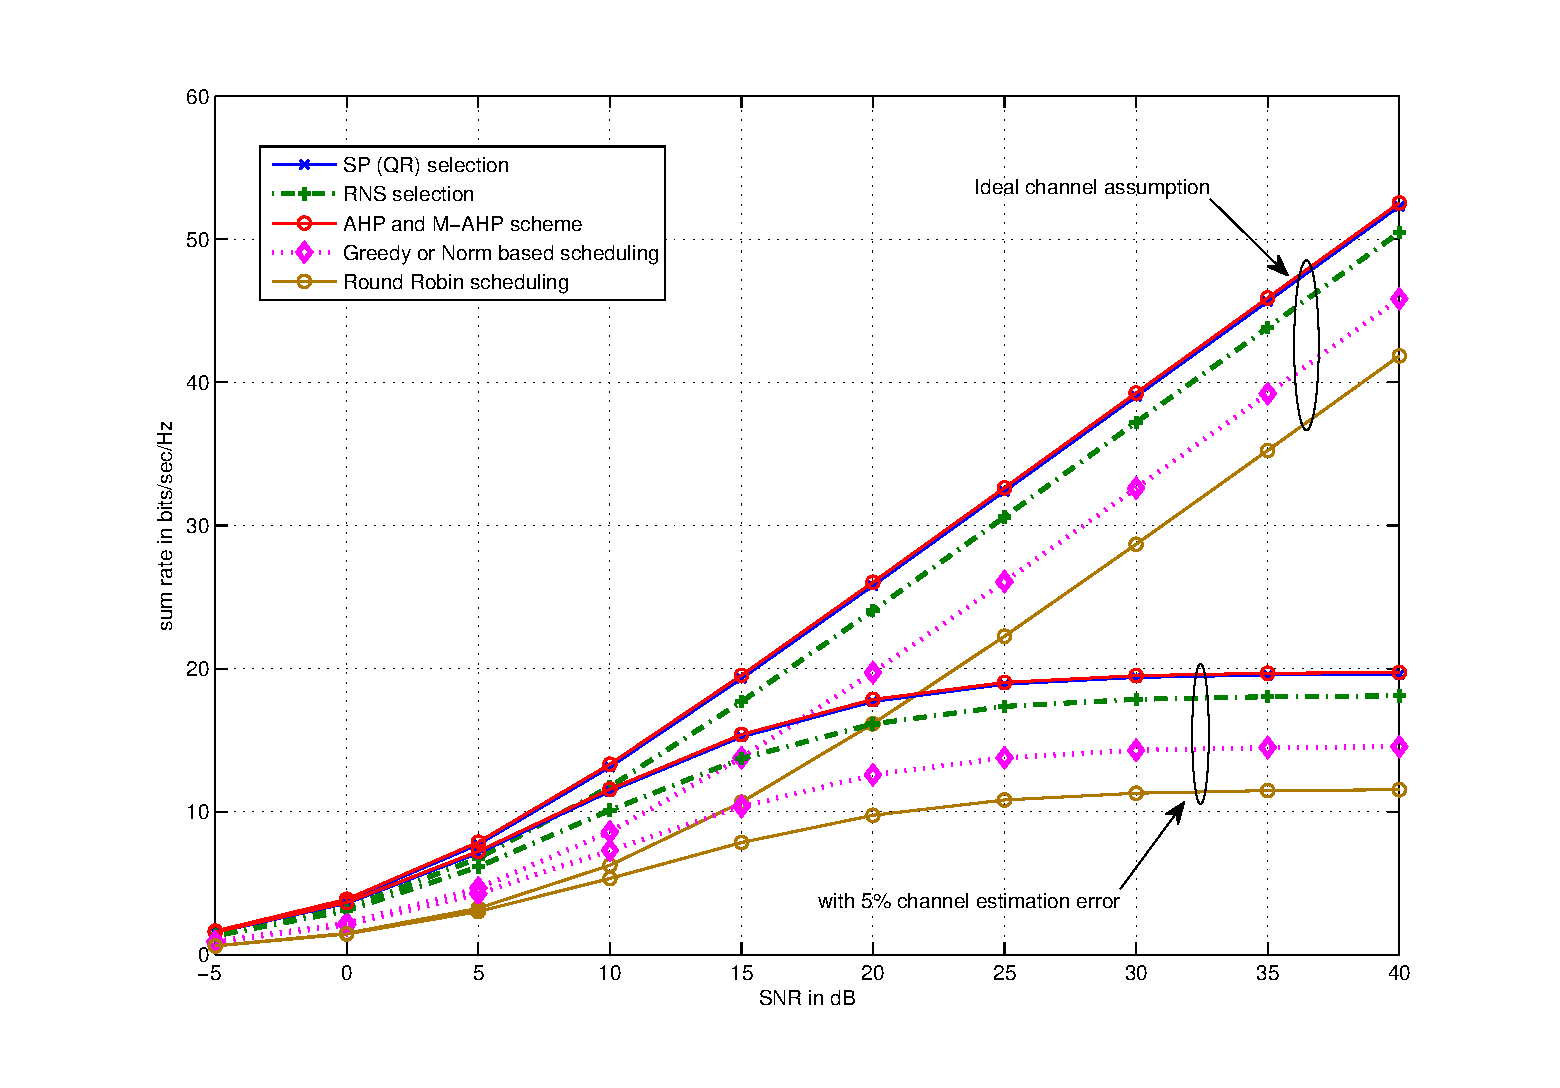
\includegraphics[width=1.0\columnwidth]{single-bs-7}
\vspace{-0.2in}
\caption[short]{Sum rate for \me{\card{\mc{U}} = 20, \, N_\mrm{T} = 4, \, N_\mrm{R} = 1}}
\vspace{-0.1in}
\label{single-bs-f1}
\end{figure}

Fig. \ref{single-bs-f1} compares the sum rate plot attained by scheduling schemes discussed so far. The \ac{AHP} scheme, which selects the user by considering not only the existing set of users \me{\mc{S}} but also the other users in the set \me{\mc{U} \bs \mc{S}}, performs noticeably better than the SP based scheme.  The gain achieved is not significant when compared with the complexity involved in the selection procedure. Fig. \ref{single-bs-f1} also shows the performance of the \ac{RNS} based selection scheme, which performs marginally close to the SP scheme with a significant reduction in the complexity. The \ac{RR} and norm based scheduling are also compared for illustrative purposes along with the \ac{SP} scheme. The figure also shows the gain degradation in the presence of estimation error in the channel. Adding estimation error of \me{5\%}, degrades the sum rate noticeably. For example, at \me{25} dB SNR, the loss is almost \me{10} bits with the estimation error. The performance loss is mainly attributed to the interference leakage by the \ac{ZF} precoder when the channel used is imperfect at the transmitter.
\begin{figure}
\centering
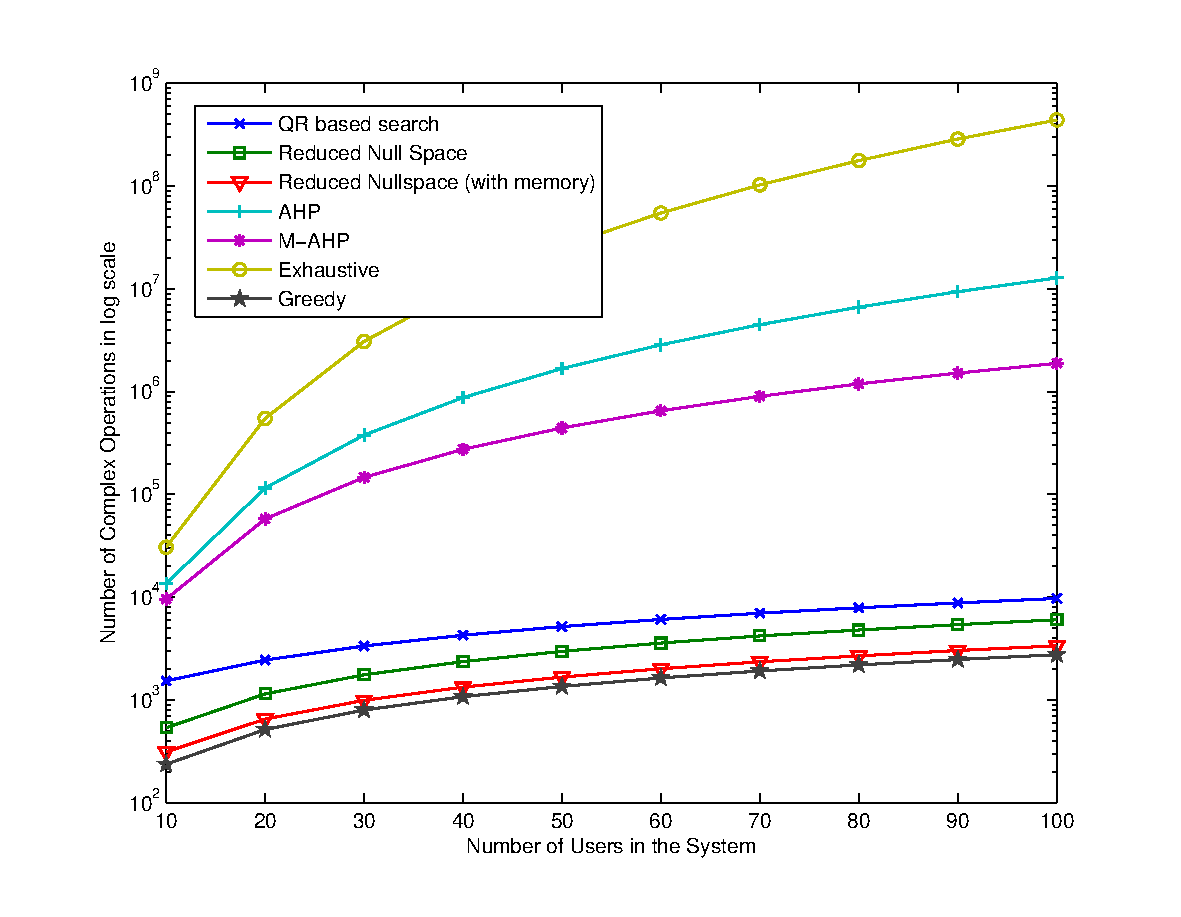
\includegraphics[width=1.0\columnwidth]{single-bs-6}
\vspace{-0.2in}
\caption[short]{Scaling of complexity over users for \me{N_\mrm{T} = 4, \, N_\mrm{R} = 1} system}
\vspace{-0.1in}
\label{single-bs-f2}
\end{figure}

Fig. \ref{single-bs-f2} compares the complexity involved in the metric calculation for different scheduling schemes with the number of users being the variable. The complexity involved with the \ac{AHP} based selection scheme is of polynomial order due to \me{K \frac{(K + 1)}{2}} pairs involved in the computation. The \ac{RNS} selection performs marginally inferior to the SP scheme, which requires more complex computations for the metric calculation as shown in Fig. \ref{single-bs-f2}. The \ac{RNS} scheme can be reduced further when the memory is utilized to save the earlier projections over the normalized channels in the set \me{\mc{S}}.

Fig. \ref{single-bs-f3} compares the sum rate performance of the above discussed scheduling schemes with different numbers of users. It is evident that the \ac{AHP} and \ac{M-AHP} schemes perform better over other schemes. The performance of \ac{RNS} performs close with the SP based selection with reduced complexity involved in evaluating the metric for the selection. As the number of users increases, the complexity of all scheduling schemes increases linearly except that of the \ac{AHP} scheme, which is of polynomial order. As the number of users in the system increases, the rate loss between the \ac{SP} scheme and the \ac{RNS} scheme reduces as shown in Fig. \ref{single-bs-f3}. The \ac{RNS} scheme provides two-fold benefits by reducing the load on the processor and also performs closer to the other near-optimal schemes.
\begin{figure}
\centering
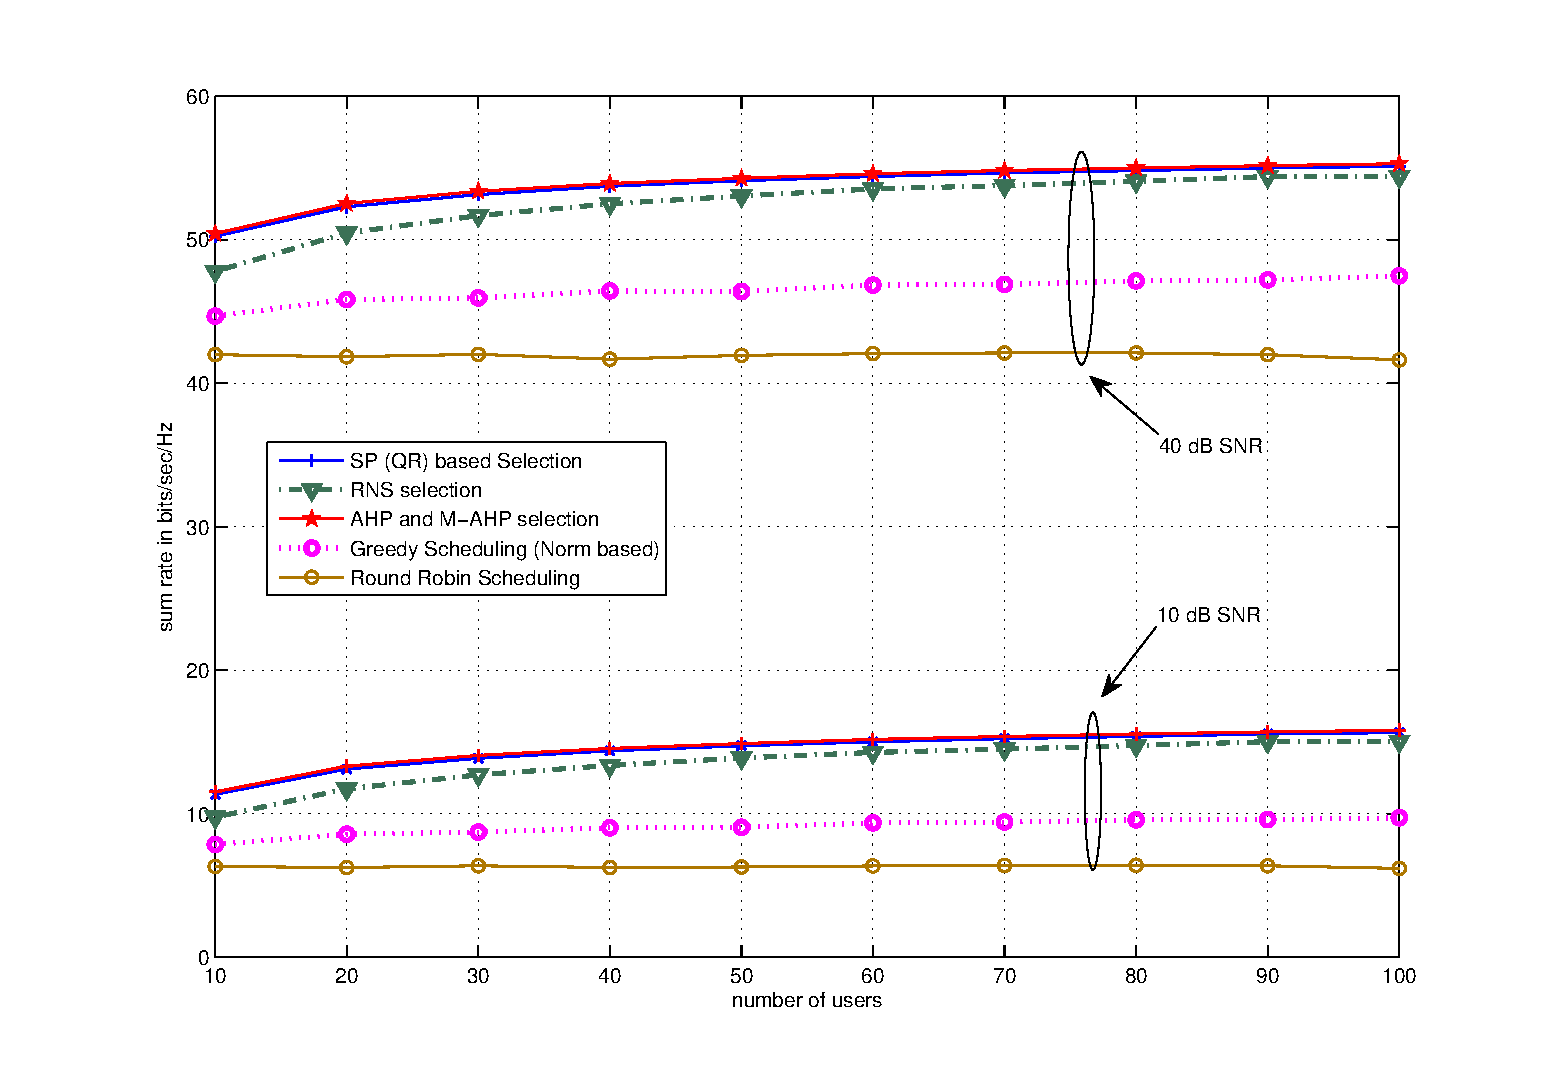
\includegraphics[width=1.0\columnwidth]{single-bs-5}
\vspace{-0.2in}
\caption[short]{Sum rate with \me{N_\mrm{T} = 4, \, N_\mrm{R} = 1} with variable users}
\vspace{-0.1in}
\label{single-bs-f3}
\end{figure}


%\subsection{Multi BS-US}


This section discusses the performance of the proposed scheduling schemes with the \ac{WSRM} objective. The proposed schemes are compared with the \ac{W-MMSE} scheme which select the users implicitly by forcing the precoder powers to zero when the users are greater than the available \ac{DoF} (overloaded \ac{W-MMSE}). We considered the cell-edge scenario for comparison. The proposed schemes are not optimal when the in-cell users are considered due to the dimensional limitation \me{\mu} discussed earlier which restricts the available \ac{DoF} in the system.
\begin{figure}
\centering
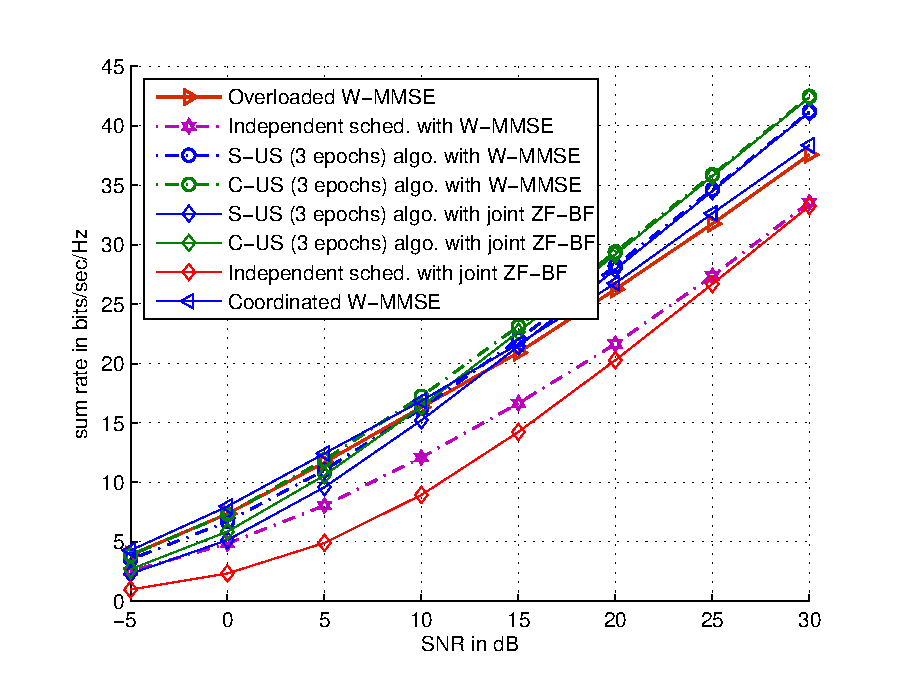
\includegraphics[width=1.0\columnwidth]{multi-bs-1}
\caption[short]{sum rate for \me{N_\mrm{T} = 4, \, N_\mrm{B} = 2, \, \card{\mc{U}_k} = 20}, \, K = 40}
\label{multi-bs-f1}
\vskip -0.2in
\end{figure}

The precoders are designed either with joint \ac{ZF}-\ac{BF} \eqref{sm-e4} or \ac{W-MMSE} scheme \cite{wmmse_shi}. The independent scheduling scheme selects the users independently across each \ac{BS} without any cooperation among \ac{BS}s, but imposes the dimensional constraint \me{\mu} so as to provide interference-free transmission using the precoders. While comparing the scheduling schemes, the \ac{W-MMSE} scheme is used to design the precoders for the users already chosen by the scheduling scheme.
\begin{figure}
\centering
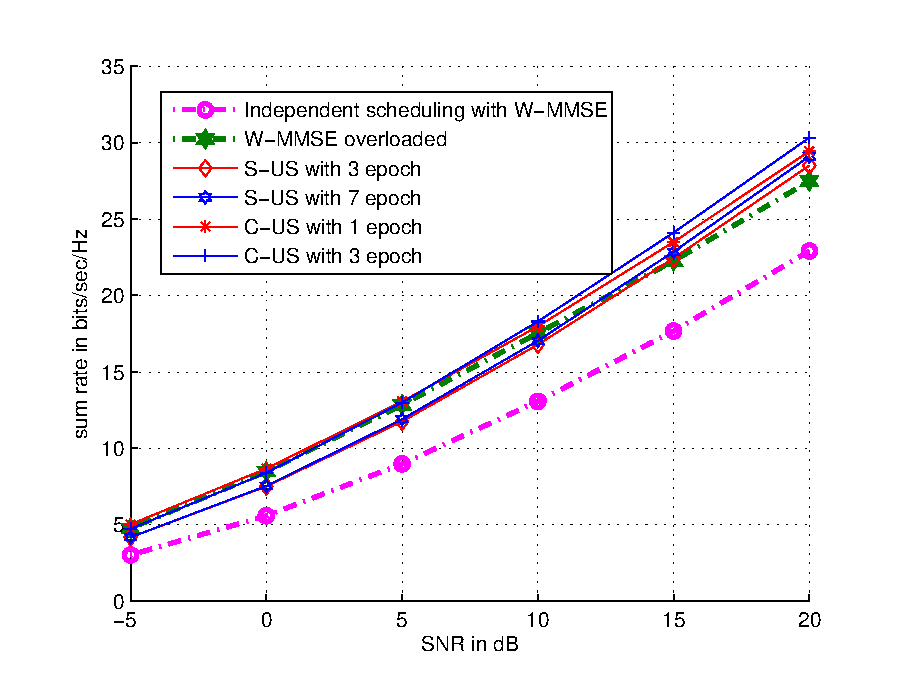
\includegraphics[width=1.0\columnwidth]{multi-bs-2}
\caption[short]{sum rate for \me{N_\mrm{T} = 4, \, N_\mrm{B} = 3, \, \card{\mc{U}_k} = 10}, \, K = 30}
\label{multi-bs-f2}
\vskip -0.1in
\end{figure}

Fig. \ref{multi-bs-f1} compares the performance of the proposed scheduling schemes. The \ac{DoF} available at each \ac{BS} is \me{N_\mrm{T} = 4} which is shared across \ac{BS}s to get \me{\mu} interference-free user streams at each \ac{BS}. The \ac{C-US} scheme performs better in comparison with the other schemes, since the users are shared across the coordinating \ac{BS}s. The sum rate achieved by \ac{C-US} scheme is evidently better than the equivalent near-optimal coordinated \ac{W-MMSE} scheme which performs both \ac{BS} and user assignment jointly. In the static user assignment case, \ac{S-US} scheme performs noticeably better than the overloaded \ac{W-MMSE} scheme at the high \ac{SNR} regime. The gain of the \ac{C-US} scheme over the \ac{S-US} scheme diminishes as the number of users in the system increases to cover all possible channel realizations within the statically assigned users. The precoder design complexity is reduced with limited user set provided by the scheduling schemes. Similar performance can be achieved using \ac{ZF}-\ac{BF} based precoding scheme at the high \ac{SNR} scheme by exploiting the \ac{MU} diversity. The selection of linearly independent users supports \ac{ZF}-\ac{BF} scheme to perform as close to near-optimal \ac{W-MMSE} design.

Fig. \ref{multi-bs-f2} shows the performance of the proposed schemes when the antennas \me{N_\mrm{T}} at each \ac{BS} is not equal to the integer multiple of \me{N_\mrm{B}}. The number of users shared equally among each \ac{BS} are given by \me{\lfloor \, \sfrac{N_\mrm{T}}{N_\mrm{B}} \, \rfloor}. The additional users as given by \me{\mod (N_\mrm{T},N_\mrm{B})} are shared across \ac{BS}s randomly to improve the multiplexing gain. The users are divided as \me{\lfloor \, \sfrac{N_\mrm{T}}{N_\mrm{B}} \, \rfloor + 1} for randomly chosen \me{\mod (N_\mrm{T},N_\mrm{B})} \ac{BS}s and the remaining \ac{BS}s with \me{\lfloor \, \sfrac{N_\mrm{T}}{N_\mrm{B}} \, \rfloor} users at a scheduling instant.

\begin{figure}
\centering
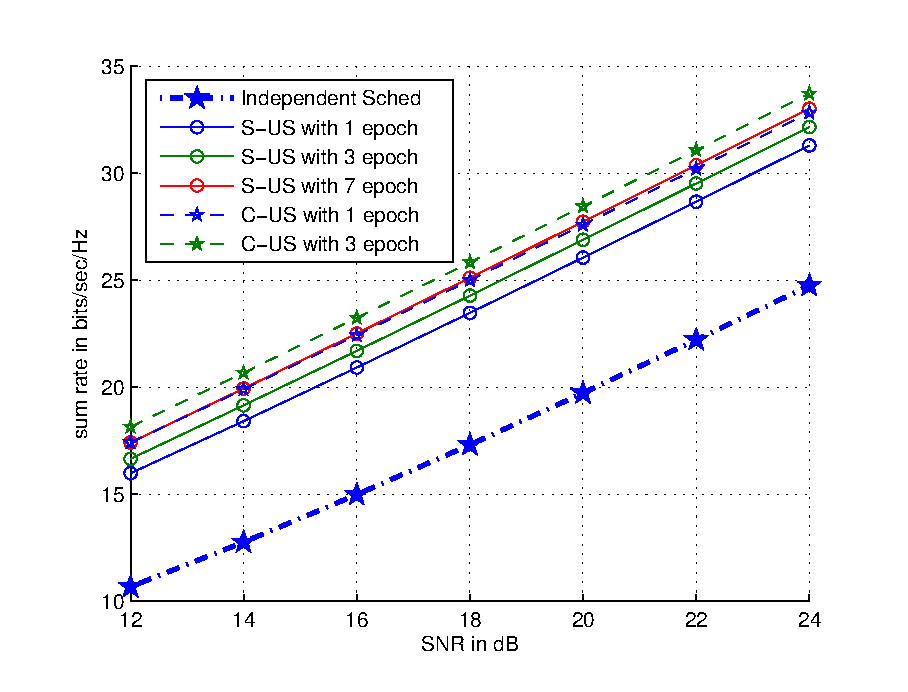
\includegraphics[width=1.0\columnwidth]{multi-bs-3}
\caption[short]{Iterative performance with \me{N_\mrm{T} = 4, \, N_\mrm{B} = 2, \, \card{\mc{U}_k} = 10}, \, K = 20}
\label{multi-bs-f3}
\vskip -0.2in
\end{figure}
The Fig. \ref{multi-bs-f3} portrays the performance improvement of the proposed scheduling schemes over multiple epochs. At each epoch, the sum rate is increased monotonically, for example, \ac{S-US} scheme achieves \me{\approx 2.5} bits by performing multiple epochs. The convergence of the \me{\mc{S}_b \fall b \inm \mc{B}} is not guaranteed to be globally optimal, since the metric used is based on null space projections which itself varies based on the chosen users channel vectors. The complexity reduction of the proposed schemes along with the precoder design is of significant importance, since the precoders are designed for the scheduled users only instead doing for all users in the overloaded \ac{W-MMSE} scenario.




\acresetall

\section{Conclusions}


The paper addressed the scheduling of users at the cell-edge in a multi-cell environment using \ac{MU} \ac{MIMO} as the transmission scheme. We proposed \ac{S-US} scheme which selects the users for each \ac{BS} jointly in an iterative manner. The \ac{S-US} scheme performs user selection by considering the interference caused to the neighboring cell users in addition to the users already chosen in the selecting \ac{BS}. The \ac{C-US} scheme which is the generalization of \ac{S-US} scheme selects the users and the \ac{BS}s jointly over the global user set. The performance improvement of the existing schemes were significantly better than the near-optimal overloaded \ac{W-MMSE} design. The complexity of designing the precoders is also greatly reduced by doing pre-selection based on the proposed scheduling schemes using
\ac{W-MMSE} or \ac{ZF}-\ac{BF} design.




\bibliographystyle{./../Templates/IEEEtranBST2/IEEEtranS}
\bibliography{./../Library/kirja_survey}

\end{document}
